\chapter{手机主题推荐系统分析}

	\section{引言}
		推荐系统的主要任务是给每个用户提供一个候选推荐列表,过程分为两步:1、预测用户会对哪些物品评分,2、预测用户会给该物品什么评分。本章首先介绍推荐系统的目标,然后详细介绍手机主题推荐系统的排序模块,排序模块的本质就是预测用户会对哪些物品做出多少评分。
		
		在推荐过程中会遇到诸如冷启动问题、数据稀疏性问题,引入了用户画像就为解决这些问题:推荐系统首先利用用户画像模型中兴趣需求信息和推荐主题模型中的特征信息匹配,然后使用相应的推荐算法进行计算筛选,找到用户可能感兴趣的推荐主题,最后推荐给用户。

		除此之外还有一个关注点就是推荐系统的长尾性和时效性,长尾效应对提高商品销售量有非常大的帮助,而推荐的时效性对于用户的体验度也很重要,比较常见的时间效应问题主要反映在用户兴趣的变化、物品流行度的变化以及手机主题的季节效应。用户兴趣探索则是其中比较有效的解决途径之一,因为度量用户对物品的喜好不仅取决于用户的喜好和物品的属性,也取决于用户所处的环境,或者称做上下文。用户在不同的时间可能喜欢不同的物品,物品在不同的时间也有不同的流行度。因此推荐系统应该是一个动态系统,随着时间的变化会给用户不同的推荐结果\citep{temporal-cf}。

	\section{手机主题推荐系统引擎模块}
		\subsection{推荐系统的目标}
		手机主题推荐系统的目标,首先是要帮助用户快速找到所需。推荐系统作为手机主题应用平台的重要组成部分,其目标就是为用户快速找到“高品质,低价格”的商品,衡量目标是否实现就看用户看了推荐结果以后的下单转化效果。另外,推荐系统希望用户对其的认知是“无所不有”的大平台,所以也希望推荐出来的结果包含多个类型的结果,即推荐结果有多样性。目前,推荐系统的目标还主要集中在下单转化效果,随着下单率效果的大幅度提高会逐渐把重心转到多样性。
		\subsection{推荐系统框架总览}
		推荐系统框架总览如\autoref{pic:hl_recmd_structure2}。
		\begin{figure}
	    \centering
	      \framebox{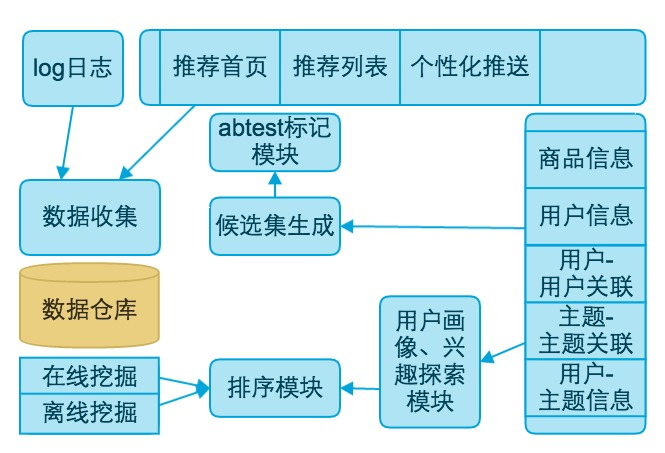
\includegraphics[scale=0.6]{figures/hl_recmd_structure2}}
	      \figcaption{推荐系统引擎框架总览图}
	      \label{pic:hl_recmd_structure2}
	    \end{figure}

		最顶层显示的是推荐系统对外的服务接口。由于不同展位的输入输出参数差异较大,因此这一层没有做过多的抽象,每个展位有自己特定的接口形式。接口层会调用abtest配置模块,对接入的流量按照uuid、城市等维度进行分流量的配置。Abtest配置模块之下,是推荐候选集的生成,排序和业务处理模块。候选集生成和排序模块,除了针对不同展位有不同逻辑以外,对同一展位的不同策略也有不同的逻辑。abtest模块在配置流量策略的时候,可以根据需要单独配置候选集策略和排序策略。从接口层接受到的每次响应请求会打印一些必要的日志,记录这次请求的一些必要的上下文信息以及用户及item相关的特征信息,以便生成用户行为数据。这些日志通过flume传输到HDFS上面。借助Hadoop、Hive、Spark等平台对原始日志进行处理,从而得到需要的各种数据及模型:包括用户的画像信息,用户之间的相似度,item之间的相似度。在推荐系统的候选集生成这一块,重度使用了传统的user based,item based协同过滤算法,协同过滤算法需要在用户行为较丰富的情况下才能奏效。而对于那些行为稀少的用户,需要根据平台的特点进行做好冷启动策略。这里面需要注意的是,推荐系统引入了时间衰减的因子,从而使新的行为起的作用大于老的行为,从结果来看确实对于效果会有提升。
		\subsection{排序模块}
		对于推荐系统的效果提高,排序比候选集的贡献要大很多。排序方面所做的主要工作:
		\begin{enumerate}[(1)]
			\item 模型及建模

			目前的推荐系统的排序模型主要是Additive Groves模型。AG模型是一种决策树类型的模型,属于非线性模型。这种非线性模型的特点,是一定程度上能够自动进行特征组合的工作,不需要人工进行大量这类工作。建模方法和传统的ctr预估建模方法一样,是point wise的模型。每一个item对一个用户的每次展示可以作为一个样本,这个item是否被点击或者是否被下单作为标记。推荐系统会为这些样本抽取一些item特征,用户特征,上下文特征,item与用户的交叉特征。
			\item 样本采样及label处理

			由于推荐系统的最终目标是提高item的下单转化效果,所以需要重点采用用户下单行为作为标记。但是如果只用下单行为,又会导致数据较为稀疏,有很大比例的用户很长时间内是没有下单行为的。所以我们还需要使用点击行为作为标记。而对点击行为和下单行为对于训练目标的价值是不一样的,对它们需要做不同的处理。推荐系统尝试了2种方式,在参数取得比较合适的情况下,二者的结果效果都很好。一种方式是提高下单样本的采样比例。一种方式是提高标记值。比如下单行为的标记值为30,点击行为的标记值为1。
			\item 去除position bias

			item在展示列表中的位置,对item的点击概率和下单概率是有非常大影响的,排名越靠前的item,越容易被点击和下单,这就是position bias的含义。在抽取特征和训练模型的时候,就需要很好去除这种position bias。推荐系统在两个地方做这种处理:一个是在计算item的历史平均点击率ctr(Click-Through-Rate)和历史平均下单率cvr(Click Value Rate)的时候,首先要计算出每个位置的$ctr_p$和率$cvr_p$,然后在计算item的每次点击和下单的时候,都根据这个item被展示的位置,计算为$ctr_0$/$ctr_p$及$cvr_0$/$ctr_p$;一个是在产生训练样本的时候,把展示位置作为特征放在样本里面,并且在使用模型的时候,把展示位置特征统一置为0。
			\item 特征工程

			特征工程是排序模型的最重要工作,排序带来的效果提升,大部分是由特征工程带来的。特征提取就是不断地去接触和理解业务数据,试图从中挖掘出和用户转化相关的特征。使用的主要特征包括:上下文特征:如时间,地理位置,天气,温度等。item特征:如团购服务的价格,销量,用户评分。用户特征:用户的属性特征,如年龄,性别,婚育状态,品类偏好,价格偏好等。
		\end{enumerate}

	\section{用户画像模块}
		\subsection{用户画像介绍}
		用户画像模型,用户兴趣探索模块,推荐系统模块之间的关系如\autoref{pic:hl_iterate}。
		\begin{figure}
		\centering
		\framebox{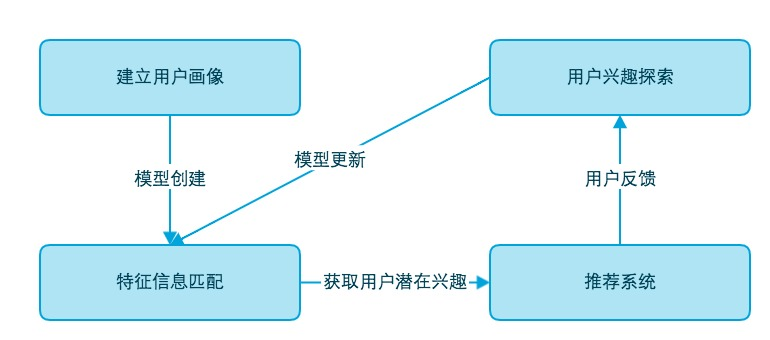
\includegraphics[scale=0.4]{figures/hl_iterate}}
		\figcaption{手机主题推荐系统功能模块图}
		\label{pic:hl_iterate}
		\end{figure}

		目前基于用户画像的推荐,主要用在基于内容的推荐,从最近的RecSys大会(ACM Recommender Systems)上来看,不少公司和研究者也在尝试基于用户画像做Context-Aware的推荐。利用用户的画像,结合时间、天气等上下文信息,给用户做一些更加精准化的推荐是一个不错的方向。一个好的推荐系统要给用户提供个性化的、高效的、动态准确的推荐,那么推荐系统应能够获取反映用户多方面的、动态变化的兴趣偏好,推荐系统有必要为用户建立一个用户兴趣探索模型,该模型能获取、表示、存储和修改用户兴趣偏好,能进行推理,对用户进行分类和识别,帮助系统更好地理解用户特征和类别。推荐系统根据用户画像进行推荐,所以用户画像对推荐系统的质量有至关重要的影响。建立用户画像模型之前需要考虑问题有:模型的输入数据有哪些,如何获取模型的输入数据;如何考虑用户的兴趣及需求的变化;建模的对象是谁以及如何建模;模型的输出是什么。用户画像模型的输入数据主构成包括:
		\begin{itemize}
		\item 用户属性,分为社会属性和自然属性,包括用户最基本的如用户的姓名、年龄、职业、收入、学历等信息。用户注册时的对自然属性和社会属性进行初始建模。 
		\item 用户手工输入的信息:是用户主动输出给系统的信息,包括用户在搜索引擎中打出的关键词,用户评论中发布的感兴趣的主题、频道。还有一类重要的信息就是用户反馈的信息,包括用户自己对推荐结果的满意程度;用户标注的浏览页面的感兴趣、不感兴趣或感兴趣的程度等。
		\item 用户的浏览行为和浏览内容:用户浏览的行为和内容体现了用户的兴趣和需求,它们包括浏览次数、频率、停留时间等,浏览页面时的操作(收藏、保存、复制等)、浏览时用户表情的变化等。服务器端保存的日志记录了用户的浏览行为和内容。
		\end{itemize}

		\subsection{用户画像数据来源}	    
	    电子商务用户画像的信息来源可以有如几种方式:
	    \begin{itemize}
	    \item 显式用户行为。显式方法主要是通过获取用户注册信息中的有关的兴趣和偏好或允许用户自己定义和修改用户画像来实现,一般获取的是用户相对静态和稳定的属性,例如:性别、年龄区间、地域、受教育程度、学校、公司等。主题应用商店本身就有比较完整的用户注册引导、用户信息完善任务、认证用户审核等,在收集和清洗用户属性的过程中,需要注意的主要是标签的规范化以及不同来源信息的交叉验证。
	    \item 隐式用户行为。隐式方法则是通过跟踪用户的行为和交互来评估和推测用户画像,一般获取的是用户更加动态和易变化的兴趣特征,首先,用户兴趣会受到环境、热点事件、季节等方面的影响,一旦这些因素发生变化,用户的兴趣容易产生迁移;其次,用户的行为多样且碎片化,不同行为反映出来的兴趣差异较大。
	    \item 第三方应用数据。一些功能性应用如微信、微博提供的第三方免注册登陆API接口,可以直接获取第三方应用账号提供的用户基本数据。
	    \item 自然语言处理技术。利用自然语言处理技术提取用户购买评价、评论语句中的关键词,作为用户画像标签的一部分。
	    \end{itemize}

	    在个性化服务的用户画像建模中,最常用的方式是将以上几种或多种方法结合起来,通过显式方式来获取静态用户信息如姓名、性别、职业等;通过隐式方式来获取动态用户信息如用户兴趣、爱好等;通过第三方登陆接口获取用户的分享、动态信息等;通过自然语言处理技术分析用户的当前心态、满意度、消费心情等。

		\subsection{用户画像构建}
		一个标签通常是人为规定的高度精炼的特征标识,如年龄段标签:25到35岁,地域标签:北京。标签有两个重要特征:语义化和短文本,人能很方便地理解每个标签含义。这也使得用户画像模型具备实际意义。能够较好的满足业务需求。如,判断用户偏好。同时,每个标签通常只表示一种含义,标签本身无需再做过多文本分析等预处理工作,这为利用机器提取标准化信息提供了便利。人制定标签规则,并能够通过标签快速读出其中的信息,机器方便做标签提取、聚合分析。所以,用户画像和用户标签为我们展示了一种朴素、简洁的描述用户信息的方法。构建用户画像是为了还原用户信息,因此数据来源于所有与用户相关的数据。对于与用户相关数据的分类,一般采用一种封闭性的分类思想。如,世界上分为两种人,一种是懂计算机的人,一种是不懂计算机的人;客户分三类,高价值客户,中价值客户,低价值客户;产品生命周期分为,投入期、成长期、成熟期、衰退期,所有的子分类将构成了类目空间的全部集合。这样的分类方式,有助于后续不断枚举并迭代补充遗漏的信息维度。不必担心架构上对每一层分类没有考虑完整,造成维度遗漏留下扩展性隐患。另外,不同的分类方式根据应用场景,业务需求的不同,也许各有道理,按需划分即可。

		用户数据类型一般划分为静态信息数据、动态信息数据两大类。静态信息数据是指用户相对稳定的信息,如图所示,主要包括人口属性、商业属性等方面数据。这类信息,自成标签,如果企业有真实信息则无需过多建模预测,更多的是数据清洗工作,因此这方面信息的数据建模不是本篇文章重点。动态信息数据是指用户不断变化的行为信息,广义上讲,一个用户打开手机应用软件,点击了一个链接,购买了一个杯子等都属于用户行为。当行为集中到互联网,乃至电商,用户行为就会聚焦很多。用户行为可以被看作用户动态信息的唯一数据来源。用户画像的目标是通过分析用户行为,最终为每个用户打上标签,以及该标签的权重。其中标签表征了用户对该内容有兴趣、偏好、需求等等。权重表征了用户的兴趣、偏好指数,也可能表征用户的需求度,可以简单的理解为可信度,概率。

		下面内容将详细介绍如何根据用户行为,构建模型产出标签、权重。一个事件模型包括:时间、地点、人物三个要素。每一次用户行为本质上是一次随机事件,可以详细描述为:什么用户,在什么时间,什么地点,做了什么事。
		\begin{itemize}
			\item 什么时间:时间包括两个重要信息,时间戳+时间长度。时间戳,为了标识用户行为的时间点,通常采用精度到秒的时间戳即可。浏览器时间精度,准确度最多也只能到毫秒。时间长度为了标识用户在某一页面的停留时间。
			\item 什么地点:用户的接触点。对于每个用户接触点。潜在包含了两层信息:网址和内容。网址定位了一个互联网页面地址,或者某个产品的特定页面。可以是PC上某电商网站的页面url,也可以是手机上的微博,微信等应用某个功能页面,某款产品应用的特定画面。内容可以是单品的相关信息:类别、品牌、描述、属性、网站信息等等。其中网址决定了权重;内容决定了标签。
			\item 什么事:用户行为类型,对于电商有几种典型行为:浏览、添加购物车、搜索、评论、购买、点击赞、收藏等等。不同的行为类型对于接触点的内容产生的标签信息,具有不同的权重。
		\end{itemize}

		综合上述分析,用户画像的数据模型,可以概括为下面的公式:用户标识 + 时间 + 行为类型 + 接触点,某用户因为在什么时间、地点、做了什么事。用户标签的权重还可能随时间的增加而衰减,因此定义时间为衰减因子r,行为类型、网址决定了权重,内容决定了标签,进一步转换为公式,标签权重=衰减因子×行为权重×网址子权重。

		\subsection{用户画像标签维度}
	    一个用户可以从多个方面去刻画,也就是说用户画像可以从多个维度来考虑和构建。作为虚拟电子商品交易平台,电子商务市场的用户在平台上通过某些行为(点击、浏览、购买)生产或获取信息,也通过其它一些行为(如转发、评论、赞)将信息传播出去,信息的传播是通过用户之间的社交关系所进行的,并且在生产、消费、传播信息的过程中对信息的选择和过滤体现了用户在兴趣方面的倾向性。由此,我们可以将用户画像按照\autoref{pic:hl_userDimension}所示的四个维度进行划分,即属性维度、兴趣维度、社交维度和行为维度。
	    \begin{figure}
	    \centering
	      \framebox{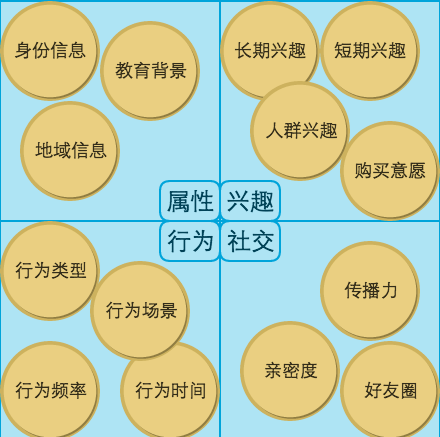
\includegraphics[scale=0.6]{figures/hl_userDimension}}
	      \figcaption{用户画像维度图}
	      \label{pic:hl_userDimension}
	    \end{figure}
	    用户属性和用户兴趣是传统用户画像中包含的两个维度。前者刻画用户的静态属性特征,例如用户的身份信息(性别、年龄、受教育程度、学校等),后者则用于刻画用户在信息筛选方面的倾向(例如用户的购买能力、兴趣标签、能力标签等)。社交维度是从社交关系及信息传播的角度来刻画用户的。在社区中用户不在仅仅是一个个体,用户和用户之间的社交关系构成了一张网络,信息在这张网络中高速流动,但是这种流动并不是无差别的,信息的起始点,所经历的关键节点以及这些节点构成的关系圈都是影响信息流动的重要因素。行为维度是一个比较新的研究方向,目的是发现影响用户属性、信息变化的行为因素,分析典型用户群体的行为模式。一方面可以通过行为模式的复用来促进用户在电子商务应用平台的成长;另一方面也有利于平台认识用户,和发现新的或异常的用户行为。属性维度:属性维度属于传统用户画像的范畴,即对用户的信息进行标签化。一方面,标签化是对用户信息进行结构化,方便计算机的识别和处理;另一方面,标签本身也具有准确性和非二义性,也有利于人工的整理、分析和统计。用户属性指相对静态和稳定的人口属性,例如:性别、年龄区间、地域、受教育程度、学校、公司等信息的收集和建立主要依靠产品本身的引导、调查、第三方提供等,在此基础上需要进行补充和交叉验证。
        \begin{itemize}
        \item 标签来源:不是所有的词都适合充当用户标签,这些词本身应该具有区分性和非二义性;此外,还需要考虑来源的全面性,除了用户主动提供的兴趣标签外,用户在使用的过程中的行为,构建的用户关系等也能够反应用户的兴趣,因此也要将其考虑在内。
        \item 权重计算:得到了用户的兴趣标签,还需要针对用户给这些标签进行权重赋值,用来区分不同标签对于该用户的重要程度。
        \end{itemize}

        兴趣维度:由于用户兴趣维度的重要性,因此有一个独立于用户画像模块的兴趣探索模块,下一章节将会详细介绍到。用户兴趣是更加动态和易变化的特征,首先兴趣受到人群、环境、热点事件、行业等方面的影响,一旦这些因素发生变化,用户的兴趣容易产生迁移;其次,用户的行为多样且碎片化,不同行为反映出来的兴趣差异较大,在用户画像建模的过程中,主要考虑如几个方面:
        \begin{itemize}
        \item 时效性:随着时间的变化,用户的兴趣会发生转移,有些兴趣会贯穿用户使用社交媒体的全过程,而有些兴趣则是受热点时间、环境因素等的影响。
        \item 长尾性:对于电商领域来讲,那些冷门的用户兴趣的总和可以和那些为数不多的大众化兴趣所占的市场份额相匹配或胜出。
        \item 兴趣和购买意愿的区分:用户具有某方面的兴趣,只代表了他愿意接受这方面的信息,并不能代表他具有购买相关内容的意愿。例如对于一些只看不买的用户,我们认为其购买意愿很小,因此对其会尽可能多的展示免费主题。
        \end{itemize}

        社交维度:如果将主题应用平台的用户视作节点,用户之间的关系视作节点之间的边,那么这些节点和边将构成一个社交的网络拓扑结构,或称作社交图谱。消费信息就是在这个图谱上进行传播。从社交的维度建立用户画像,需要从不同的角度细致和全面地描述这个消费图谱的特征,反应影响信息传播的各层面上的因素,寻找节点之间的关联度,以及刻画图谱本身的结构特征。其中包括:
        \begin{itemize}
        \item 用户个体对消费信息传播的影响:不同用户在信息传播过程中的重要性不一样,影响大的用户对于信息的传播较影响小的用户更具有促进作用。
        \item 量化用户关系紧密度:存在社交关联的用户,关系越近的用户之间越容易产生相同的消费行为。
        \item 寻找相似的用户:消费中非对等的关系本身可以认为是一种认证,用户基于兴趣、消费态度等原因反应到线上的一种关联。那么在消费维度上的相似用户至少能反应他们在某种因素上的一致性。
        \item 识别关系圈:从关系图谱的本身的结构出发,从中发掘关联紧密的群体,有助于促销广告的精准投放和主题包的推广。以上关于关系建模的任务可以看作是逐步深入的,从“个体”-->“关联”-->“相似”-->“群体”的逐渐深入。
        \end{itemize}

        行为维度:分析用户的行为,建立行为模式有两个任务:针对典型个体行为进行时序分片,分析用户成长的相关因素;针对典型群体的行为进行统计,为其构建通用的用户画像。
        \begin{itemize}
        \item 典型个体的行为时序分析。所谓典型个体是指某段时间内,成长比较突出的用户。例如从一个新用户从新注册到点击过百、浏览过千需要有一个积累过程,有些用户积累较快,有些较慢,而这些积累较快的用户可以作为典型个体;或者某些用户在某一阶段消费有限,但在某时刻消费激增,无论是消费金额还是数量都变化很大,这种也可以作为典型个体。针对典型个体,需要挖掘与其用户成长相关的行为因素。基本方法是对时间进行分片,获取用户在不同时间片上的行为统计,以及在各个时间分片上的用户成长指标(点击量、购买量、点击转换比等)。在此基础上针对用户行为的统计量的变化,利用关联性分析或回归来分析用户成长与哪些因素有关。
        \item 典型群体行为模式分析。针对典型个体,从用户的基本信息、人口信息、兴趣维度,可以将相似的典型用户划分为同一的群体,称作典型群体,针对典型群体中的用户按照成长程度进行划分,按不同的成长阶段统计用户行为,即建立了该典型群体的行为模型。例如,对于“年龄在20~30岁,女性,付费用户”这样的典型群体,从日点击量、月消费额等维度将其划分到初创、成长、快速提升、成熟等阶段,针对不同成长阶段内的行为组合进行统计,结果构成该群体的行为模式。如\autoref{pic:hl_usergroup}。
        \end{itemize}

        \begin{figure}
        \centering
          \framebox{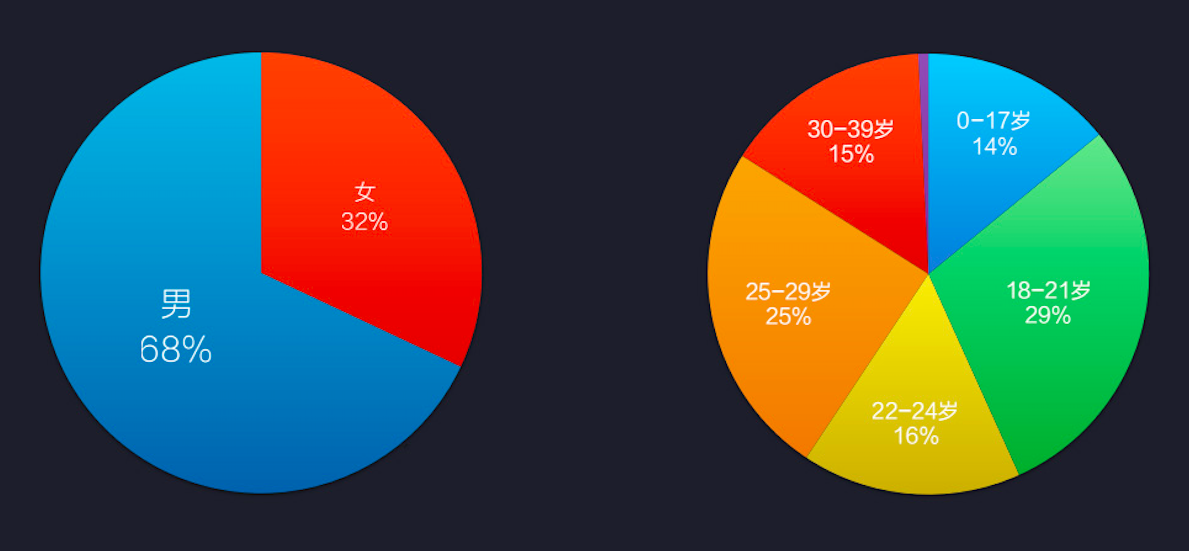
\includegraphics[scale=0.35]{figures/hl_usergroup}}
          \figcaption{电子商务用户分布图}
          \label{pic:hl_usergroup}
        \end{figure}

		\subsection{用户画像应用场景}
		\begin{enumerate}[(1)]
		\item 优化电子商务市场供求。

		改变了原有的先设计、再销售的传统模式。第三方主题设计师在设计一款新产品前,会先设定好主题类型,然后通过用户画像平台中分析该用户群体的偏好,有针对性的设计产品,从而改变原先新产品高失败率的窘境,增强销售表现。如设计一款智能手表主题,面向28-35岁的年轻男性,通过在平台中进行分析,发现属性=“金属”、风格=“硬朗”、颜色="深灰色"、价格区间=“中等”的偏好比重最大,那么就给新产品的设计提供了非常客观有效的决策依据。
				
		\item 提高新人留存率。

		工商管理有一个理论叫做,维护一个老用户的成本是获取新用户成本的五分之一甚至更低。所以如果能够把一些已经流失的用户召回来,这时候成本比拉一个新用户低得多,你做的事也会带来更大的价值。首先利用用户画像得出最近一个月没有登录过的用户数据,然后根据浏览时长分档,这是因为用户需要花自己的时间成本才能留下的最有价值的标签,之后利用用户静态标签,像姓名、职业、年龄、地域分布做进一步的细分,最后针对不同类型的用户提供不同的优惠活动。
				
		\item 用户消费等级分群。

		大至用户终端品牌、机型、操作系统,细至屏幕分辨率、屏幕尺寸,用户画像记录了每一个用户群体的详细终端特征。哪一类人群最容易被这款应用吸引,愿意为这款应用付费?开发者经常考虑的问题可以从用户画像找到答案。每一个用户群的价格分布、增值业务费用分布以及流量费用,包括用户详细的消费特征,比如付费频率,丰富了推荐系统的数据依据。
				
		\item 用户流失预警。

		一般情况用户在消费过程中会经历几个期间:新鲜期,沉迷期,消退期,离开四个阶段,如何能够延长用户在应用的停留周期是需要解决的问题之一。用户画像可以辅助推荐系统进行流失用户特征分析,通过决策数算法,分析流失用户特征,建立不同原因流失的用户模型,然后通过这些特征得到当前在应用活跃用户中匹配流失概率高的用户数据。
				
		\item 反作弊。

		用户画像会对用户的消费能力、空闲时间、信用评级等维度进行打分;利用反作弊模型通过业务方访问收集数据,供安全部门参考。
		\end{enumerate}

	\section{用户兴趣探索模块}
		现实世界的一切事物都处在变化之中。用户的兴趣、物品的属性都是在不断的变化,一个系统中每天会有大量的新用户新物品加入;时间作为一种重要的上下文信息,不同的时间用户也会有不同的兴趣,比如用户在白天和晚上的兴趣可能不同,周末和工作日的兴趣可能不同,不同的季节用户的兴趣也会有所不同。因此,合理的利用时间信息,对推荐的精准度和用户的满意度将会有很大的提升。而传统的推荐系统在设计时并没有主动的考虑到时间因素,推荐系统的动态效应表现在:
		\begin{itemize}
		\item 用户偏好随时间变化(User bias shifting):用户可能在某一天只对他喜欢的物品评分,某一天可能只对他不喜欢的物品评分。因此用户某一天的平均分是随时间变化的。
		\item 物品偏好随时间变化(Item bias shifting):物品的受欢迎程度也是随时间变化的。一款主题包在刚上线的时候的因为用户关注度小平均评分会很高,随着时间的推移,越来越多的用户参与到评分中,会使其慢慢接近真实的评分。
		\item 用户兴趣随时间变化(User preference shifting):用户在不同的时候可能有不同的兴趣,比如小孩都喜欢动漫主题包,但当他长大了可能喜欢汽车主题包。
		\item 季节效应:用户行为会受季节效应的影响。主题推荐中主要的季节效应有暑期的效应,以及一些纪念日的效应(比如国庆纪念日前后,抗日题材的主题包会受到较多的关注)。
		\end{itemize}

		为保持推荐系统的动态特性,工业界一般用数据追加的方式进行增量计算。推荐系统利用hadoop集群可以在2个小时内完成最近24小时数据的增量计算并将结果追加到现有的计算结果中,耗费的这2个小时可以用更少的时间进行增量计算并做数据追加。

		\subsection{用户行为数据存储}
		电子商务用户行为数据的特点包括:用户基数庞大。以电子商务网站淘宝网为例,注册用户往往以千万计,活跃用户达百万计;用户规模增长快。每个用户的行为数量较小。即使是活跃用户,每天最多也只能产生上百条行为记录,每年不超过十万条;用户行为的计算较为复杂。计算用户的两次登录间隔天数、反复购买的商品、累积在线时间,这些都是针对用户行为的计算,通常具有一定的复杂性;用户行为数据格式不规整,字段丢失率较高。根据用户行为数据的这些特点采用基于Hadop分布式的架构。

		\subsection{用户行为处理}
		对于用户的一些人口属性信息采用了显式方式直接获取,对于用户一些明显的兴趣偏好采用了隐式获取,对于用户潜在的兴趣偏好则通过关联技术启发式获取。显式获取用户兴趣偏好的方法是简单而直接的做法,能准确地反映用户的需求,同时所得的信息比较具体、全面、客观,结果比较可靠。缺点就是数量稀少,原因用户不太愿意花时间来向商家表达自己的喜好,并且这种方法灵活性差,答案存在异质性,当用户兴趣改变时需要用户手动更改系统中用户兴趣。同时该方法对用户不是很人性化。隐式获取法是指系统通过记录用户行为数据,通过权重排序获取用户的兴趣偏好,用户的很多动作都能暗示用户的喜好,包括查询、浏览页面和文章、标记书签、反馈信息、滑屏等。隐式的跟踪可以在建立用户画像基本数据的同时不打扰用户的正常消费活动。这种方法的缺点就是跟踪的结果未必能正确反映用户的兴趣偏好。上述获取兴趣偏好的方法有时受用户教育背景、职业和习惯等因素的限制,用户有时意识不到自己的兴趣主题,因此能为用户提供启发式信息,如领域术语抽取和相似度物品聚类,可以实现领域知识的复用,为用户间的协同提供支持,提高用户兴趣获取质量。
		
		随着电子商务市场交易规模的逐步增大,积累下来的业务数据和用户行为数据越来越多,这些用户数据往往是电子商务平台最宝贵的财富。目前在电子商务推荐系统中大量地应用到了机器学习和数据挖掘技术,例如个性化推荐、搜索排序、用户画像建模等等,为企业创造了巨大的价值。数据预处理主要工作是:
		\begin{itemize}
		\item 从原始数据,如文本、图像或者应用数据中清洗出特征数据和标注数据
		\item 对清洗出的特征和标注数据进行处理,例如样本采样,样本调权,异常点去除,特征归一化处理等过程。最终生成的数据主要是供模型直接使用。
		\end{itemize}

		根据不同业务数据的预处理方式也不同,一般来讲原始服务器日志数据脏数据的形成原因包括:缩写词不统一,数据输入错误,不同的惯用语,重复记录,丢失值,不同的计量单位,过时的编码等。相应的,数据预处理内容包括数据清理、数据集成、数据变换、数据归约、数据离散化。数据清理包括格式标准化、异常数据清除、错误纠正、重复数据的清除。对于电子商务用户数据来讲,引起空缺值的原因主要是用户设备异常造成的,有些时候是因为与其他已有数据不一致而被删除或数据的改变没有进行日志记载。根据数据空缺情况的不同有不同的处理方式:
		\begin{itemize}
		\item 忽略元组。当一个记录中有多个属性值空缺、特别是关键信息丢失时,已不能反映真实情况,它的效果非常差。
		\item 去掉属性。缺失严重时,已无挖掘意义。
		\item 人工填写空缺值。但是工作量大且可行性低。
		\item 默认值。比如使用unknown或-∞。
		\item 使用属性的平均值填充空缺值。
		\item 预测最可能的值填充空缺值。使用贝叶斯公式或判定树这样的基于推断的方法。
		\end{itemize}

		\subsection{用户行为权重排序}
		用户显式行为数据记录了用户在平台上不同的环节的各种行为,这些行为一方面用于候选集触发算法中的离线计算(主要是点击、浏览),另外一方面,这些行为代表的用户兴趣强弱不同,因此在训练重排序模型时针对不同的行为设定了不同的权重值,以更细地刻画用户的行为强弱程度。此外,用户的购买、试用等行为还作为重排序模型的交叉验证特征值,用于模型的离线训练和在线预测。负反馈数据反映了当前的结果可能在某些方面不能满足用户的需求,因此在后续的候选集触发过程中需要考虑对特定的因素进行过滤或者降权,提高用户体验;同时在重排序的模型训练中,A/B测试结果作为负例参与模型训练。用户画像是刻画用户属性的元数据,其中有些是直接获取的基础数据,有些是经过挖掘的二次数据,这些属性一方面可以用于候选集触发过程中对标签进行加权或降权,另外一方面可以作为重排序模型中的用户维度特征。通过对数据的挖掘可以提取出一些关键词,然后使用这些关键词给主题打标签,用于主题的个性化展示。

		\subsection{用户行为建模}
		当我们想基于用户行为分析来建立用户兴趣模型时,我们必须把用户行为和兴趣主题限定在一个实体域上。个性化推荐落实在具体的推荐中都是在某个实体域的推荐。对于手机主题应用市场来说,实体域包括所有的主题,背景图片,铃声,闹铃等。  用户行为。浏览,点击,下载,试用,购买,评论等都可是用户行为。本文所指的用户行为都是指用户在某实体域上的行为。比如用户在手机铃声产生的行为。用户兴趣。用户的兴趣维度,同样是限定在某实体域的兴趣,通常以标签+权重的形式来表示。比如,对于手机主题,用户兴趣向量可以是「动漫,0.6」,「体育,0.1」,「情感,0.7」等分类标签。值得一提的是,用户兴趣只是从用户行为中抽象出来的兴趣维度,并无统一标准。而兴趣维度的粒度也不固定,如「体育」,「电影」等一级分类,而体育下有「篮球」,「足球」等二级分类,篮球下有「NBA」,「CBA」,「火箭队」等三级分类。我们选取什么粒度的兴趣空间取决于具体业务模型。
		
		实际应用中,在社交网络用户的行为一般是主动进行的,例如,自行定义或选择标签,浏览页面,使用站内产品或第三方APP,发表博文或对其他博文内容的点赞或收藏,关注其他用户并将其关注的对象划分到自行设置的各用户组内等。而上述这些社交网络用户的行为能够在一定程度上反映出用户的兴趣。因此,社交网络中,可以根据用户的这些网络行为来进行用户的兴趣挖掘。该阶段是用户行为数据进行建模,以抽象出用户的标签,这个阶段注重的应是大概率事件,通过数学算法模型尽可能地排除用户的偶然行为。基于用户标签的兴趣挖掘方法。具体地,可以根据标签的具体内容,将标签归类到相应的兴趣类别后,再根据用户的自定义标签及其所属的兴趣类别,分析出用户的兴趣。

	\section{本章小结}
	用户画像模块对应着用户长期兴趣,用户兴趣探索对应着用户短期动态兴趣。短期兴趣的特点是临时、易变;长期兴趣的特点是长久、稳定;用户的短期兴趣可能会转化为长期兴趣,所以需要在推荐时综合考虑长期兴趣和短期兴趣。考虑到推荐系统的时间效应问题,将输入数据集归结为一个四元组,即{用户,物品,行为,时间},数据集可以选用比较直观的显性反馈数据集,给定用户u,物品i,时间t,预测用户u在时间t对物品i的评分r。对于该类问题的评分预测问题主要有:用户兴趣的变化,如年龄增长,从儿童长成青少年壮年;生活状态的变化,由以前的小学生到大学生;社会事件的影响如俩会等。此外还有季节效应问题,一些在春季很流行的,在夏季节未必就很流行。对于时效性的影响,每个推荐系统都有不同的演化速率,相对来说新闻更新很快,但音乐、电影的跟新却比较慢。